\documentclass[../report.tex]{subfiles}
\begin{document}
    \begin{frame}
    	\frametitle{5a1) Filtering - Radius 100}
    	\begin{table}[!htb]
        \centering
        \begin{tabular}{ c m{5cm} }
        
            \begin{minipage}{0.45\textwidth}
            \frame{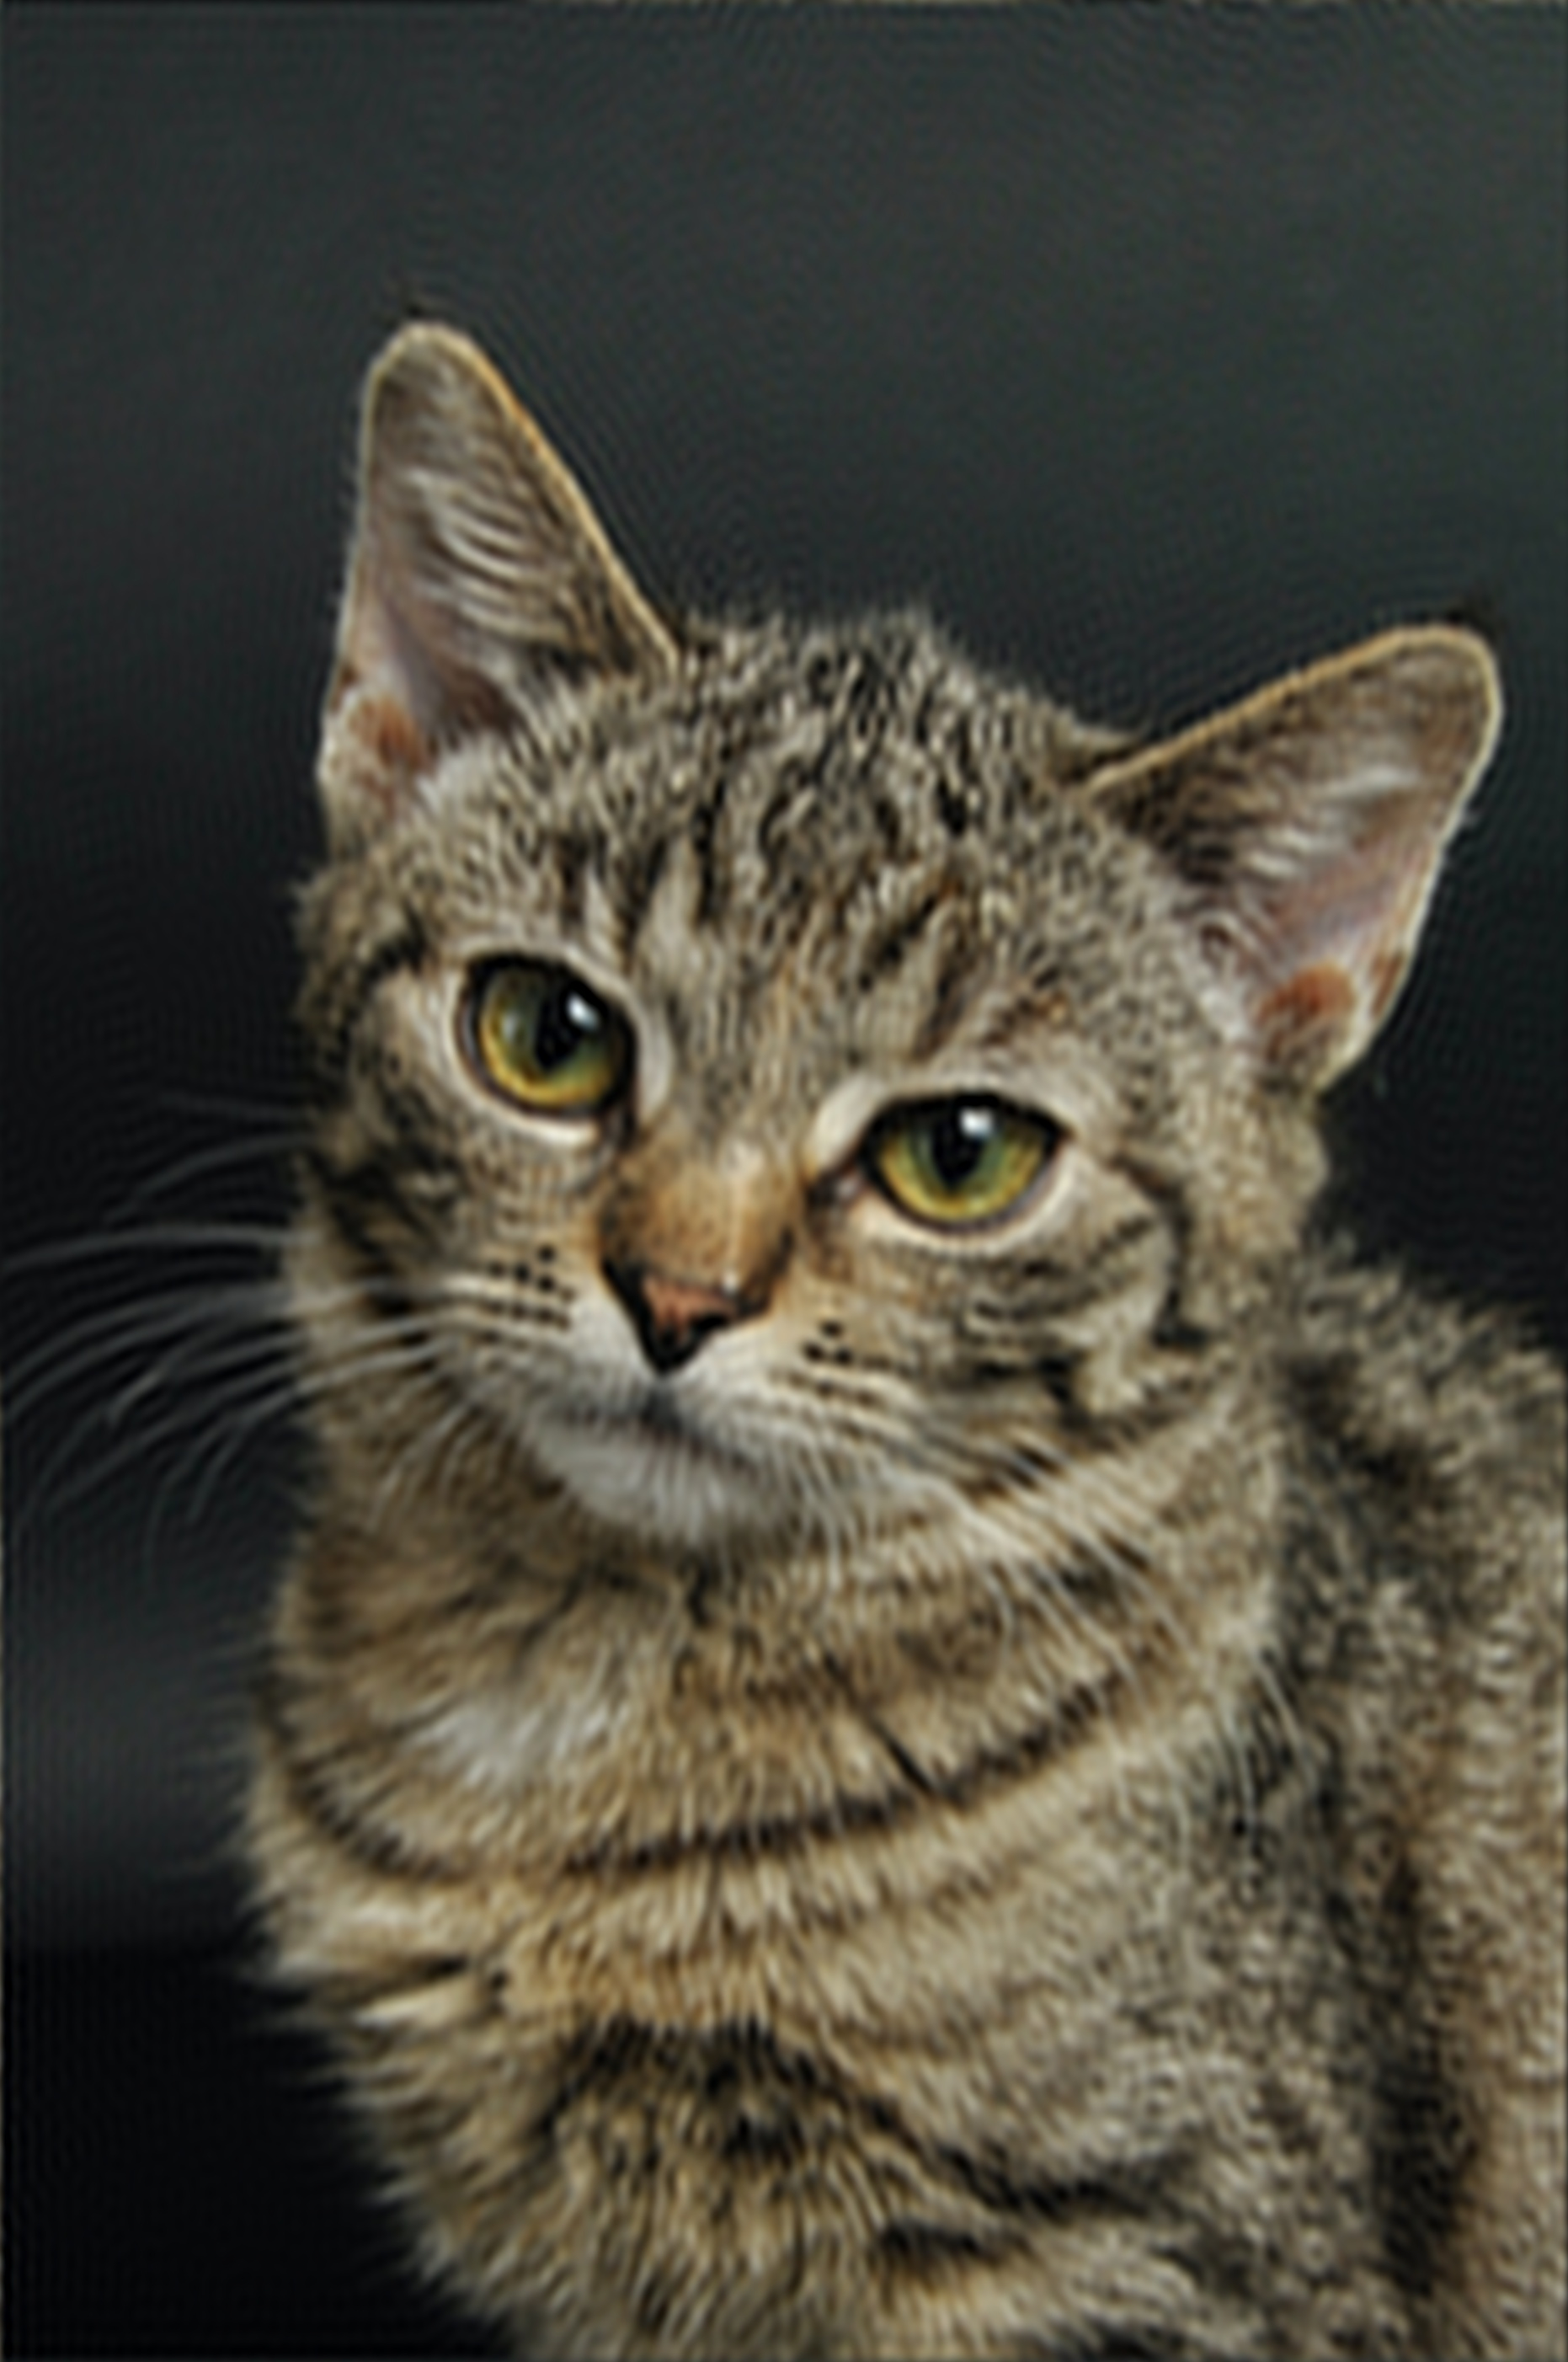
\includegraphics[keepaspectratio,height=0.7\textheight,width=1\textwidth]{output/ps2-5-a-1.jpg}}
                \captionof{figure}{ps2-5-a-1 resulting image}
            \end{minipage}
        
        	\begin{minipage}{0.45\textwidth}
        		\frame{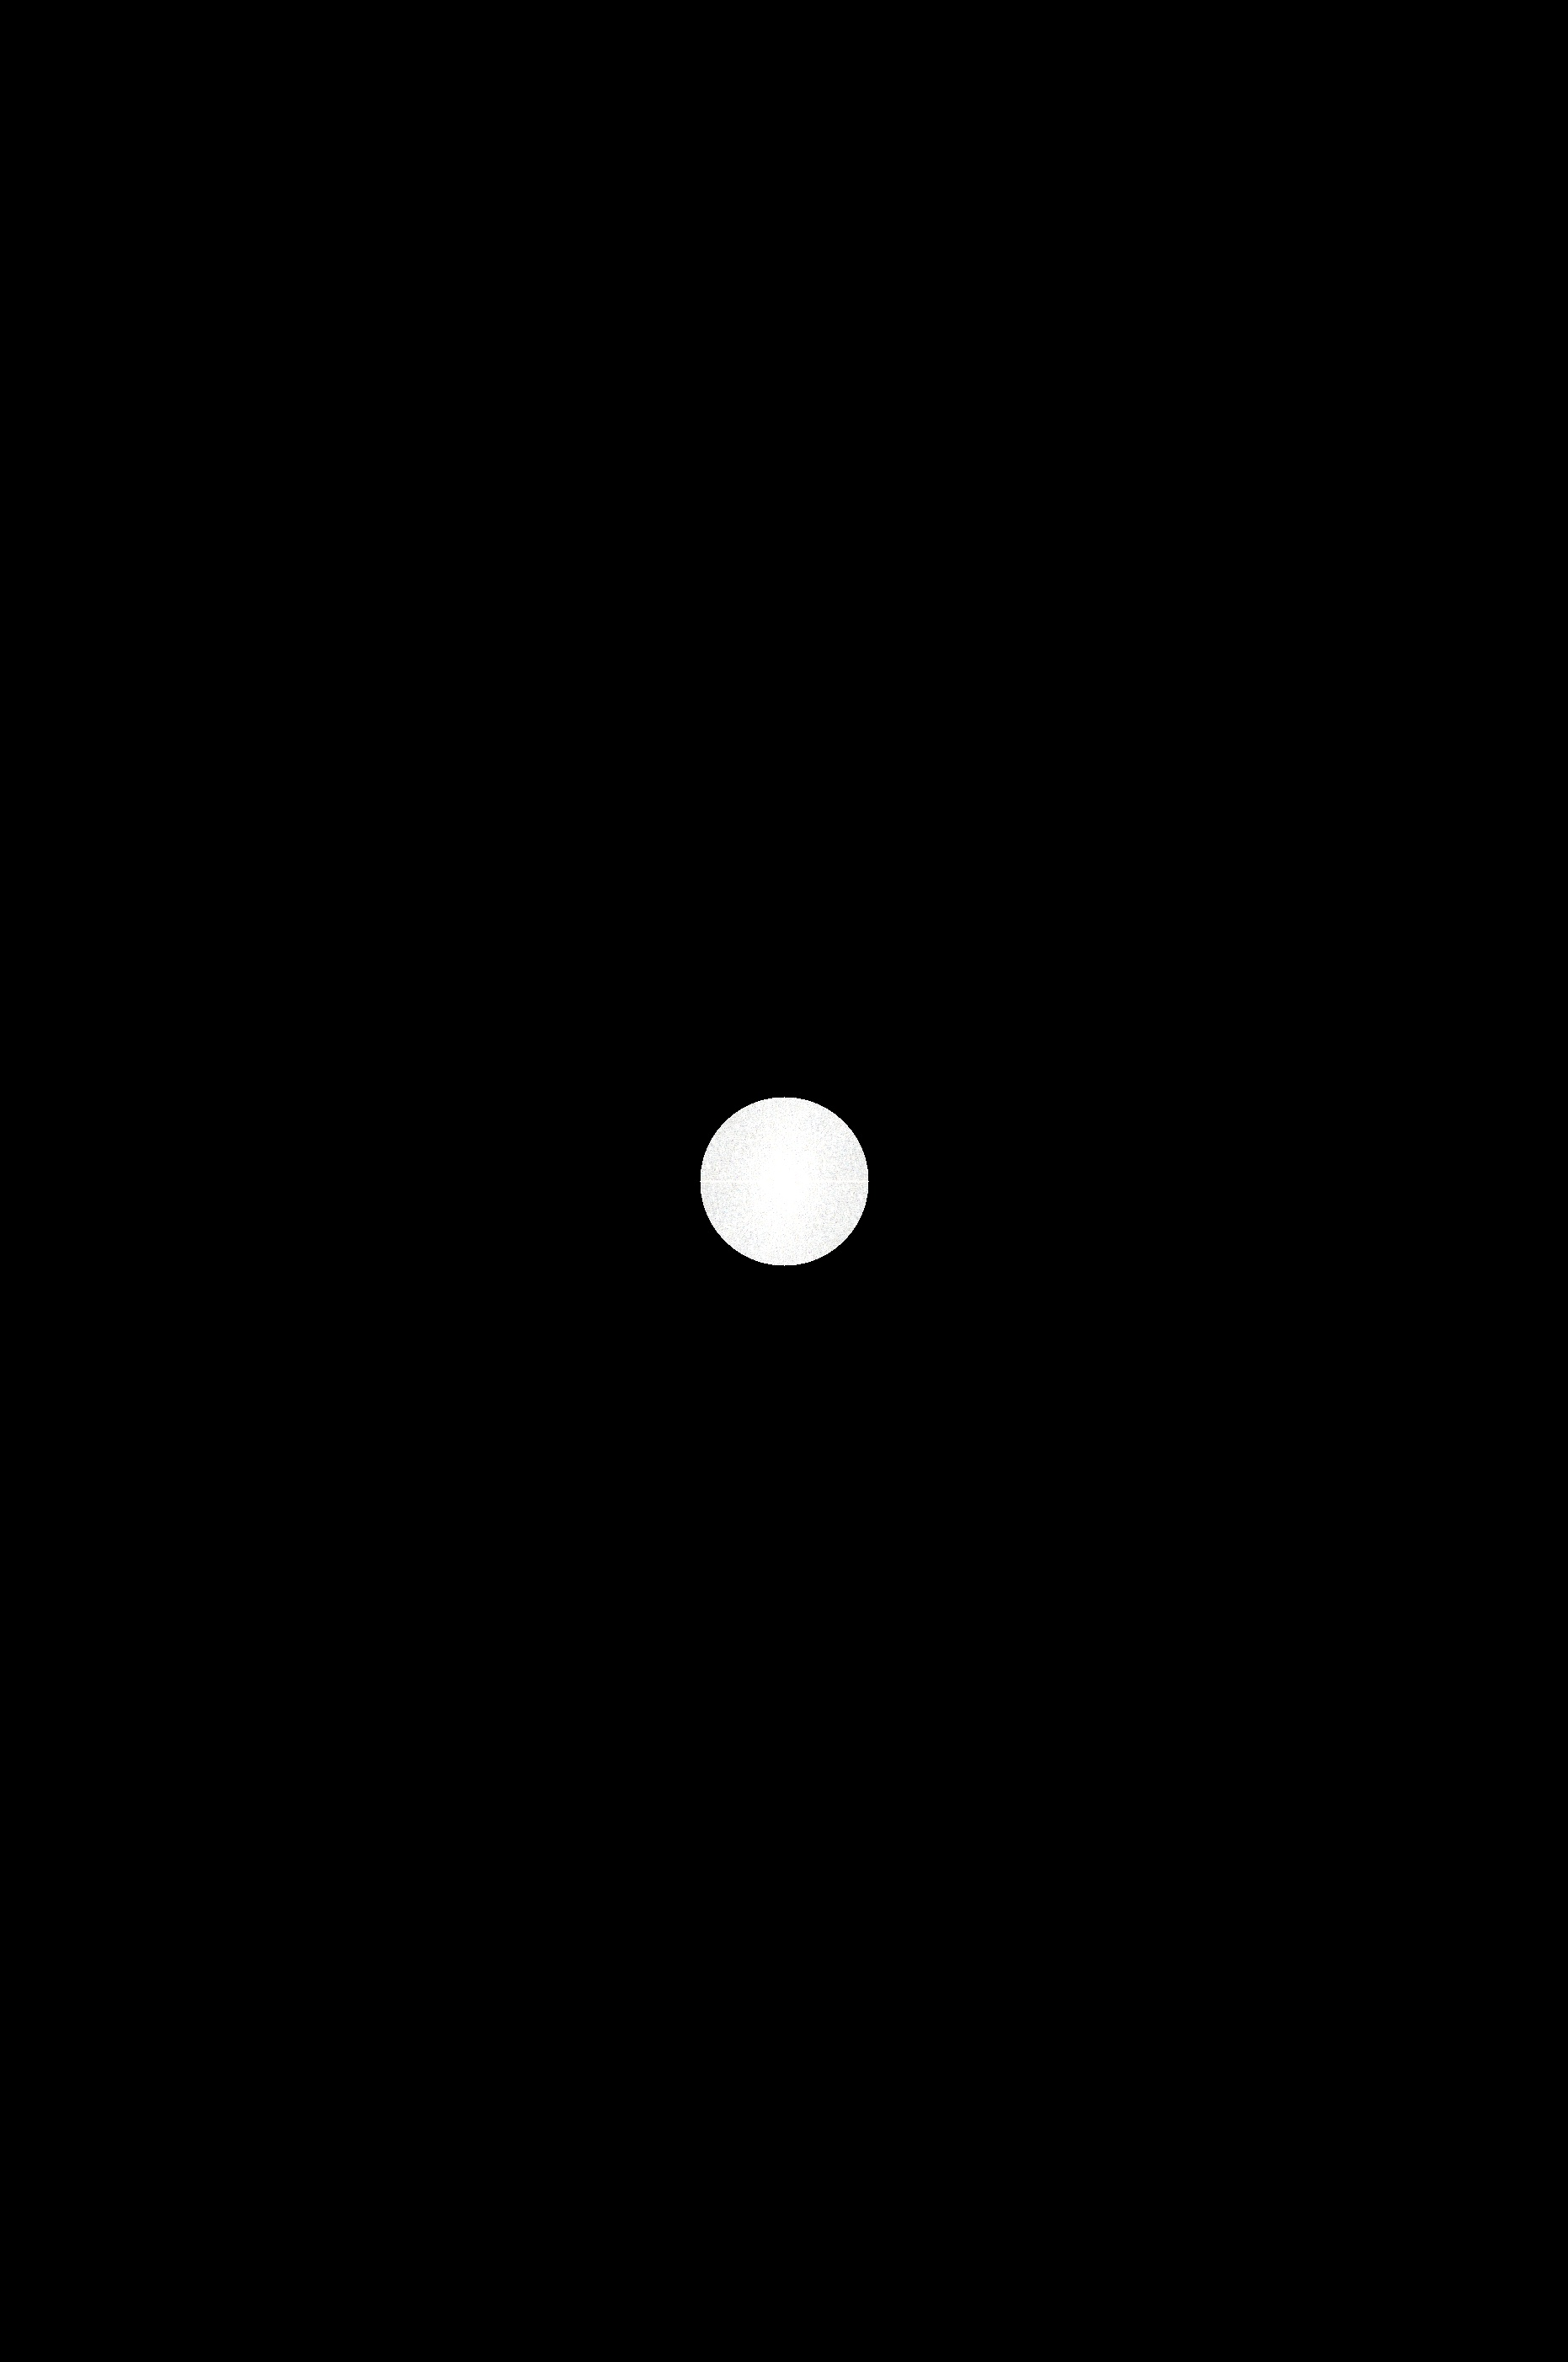
\includegraphics[keepaspectratio,height=0.7\textheight,width=1\textwidth]{output/ps2-5-a-1-freq.jpg}}
        		\captionof{figure}{ps2-5-a-1 frequency domain}
        	\end{minipage}
        
        \end{tabular}
        \end{table}
    \end{frame}
    
    \begin{frame}
    	\frametitle{5a2) Filtering - Radius 50}
    	\begin{table}[!htb]
        \centering
        \begin{tabular}{ c m{5cm} }
        
            \begin{minipage}{0.45\textwidth}
            \frame{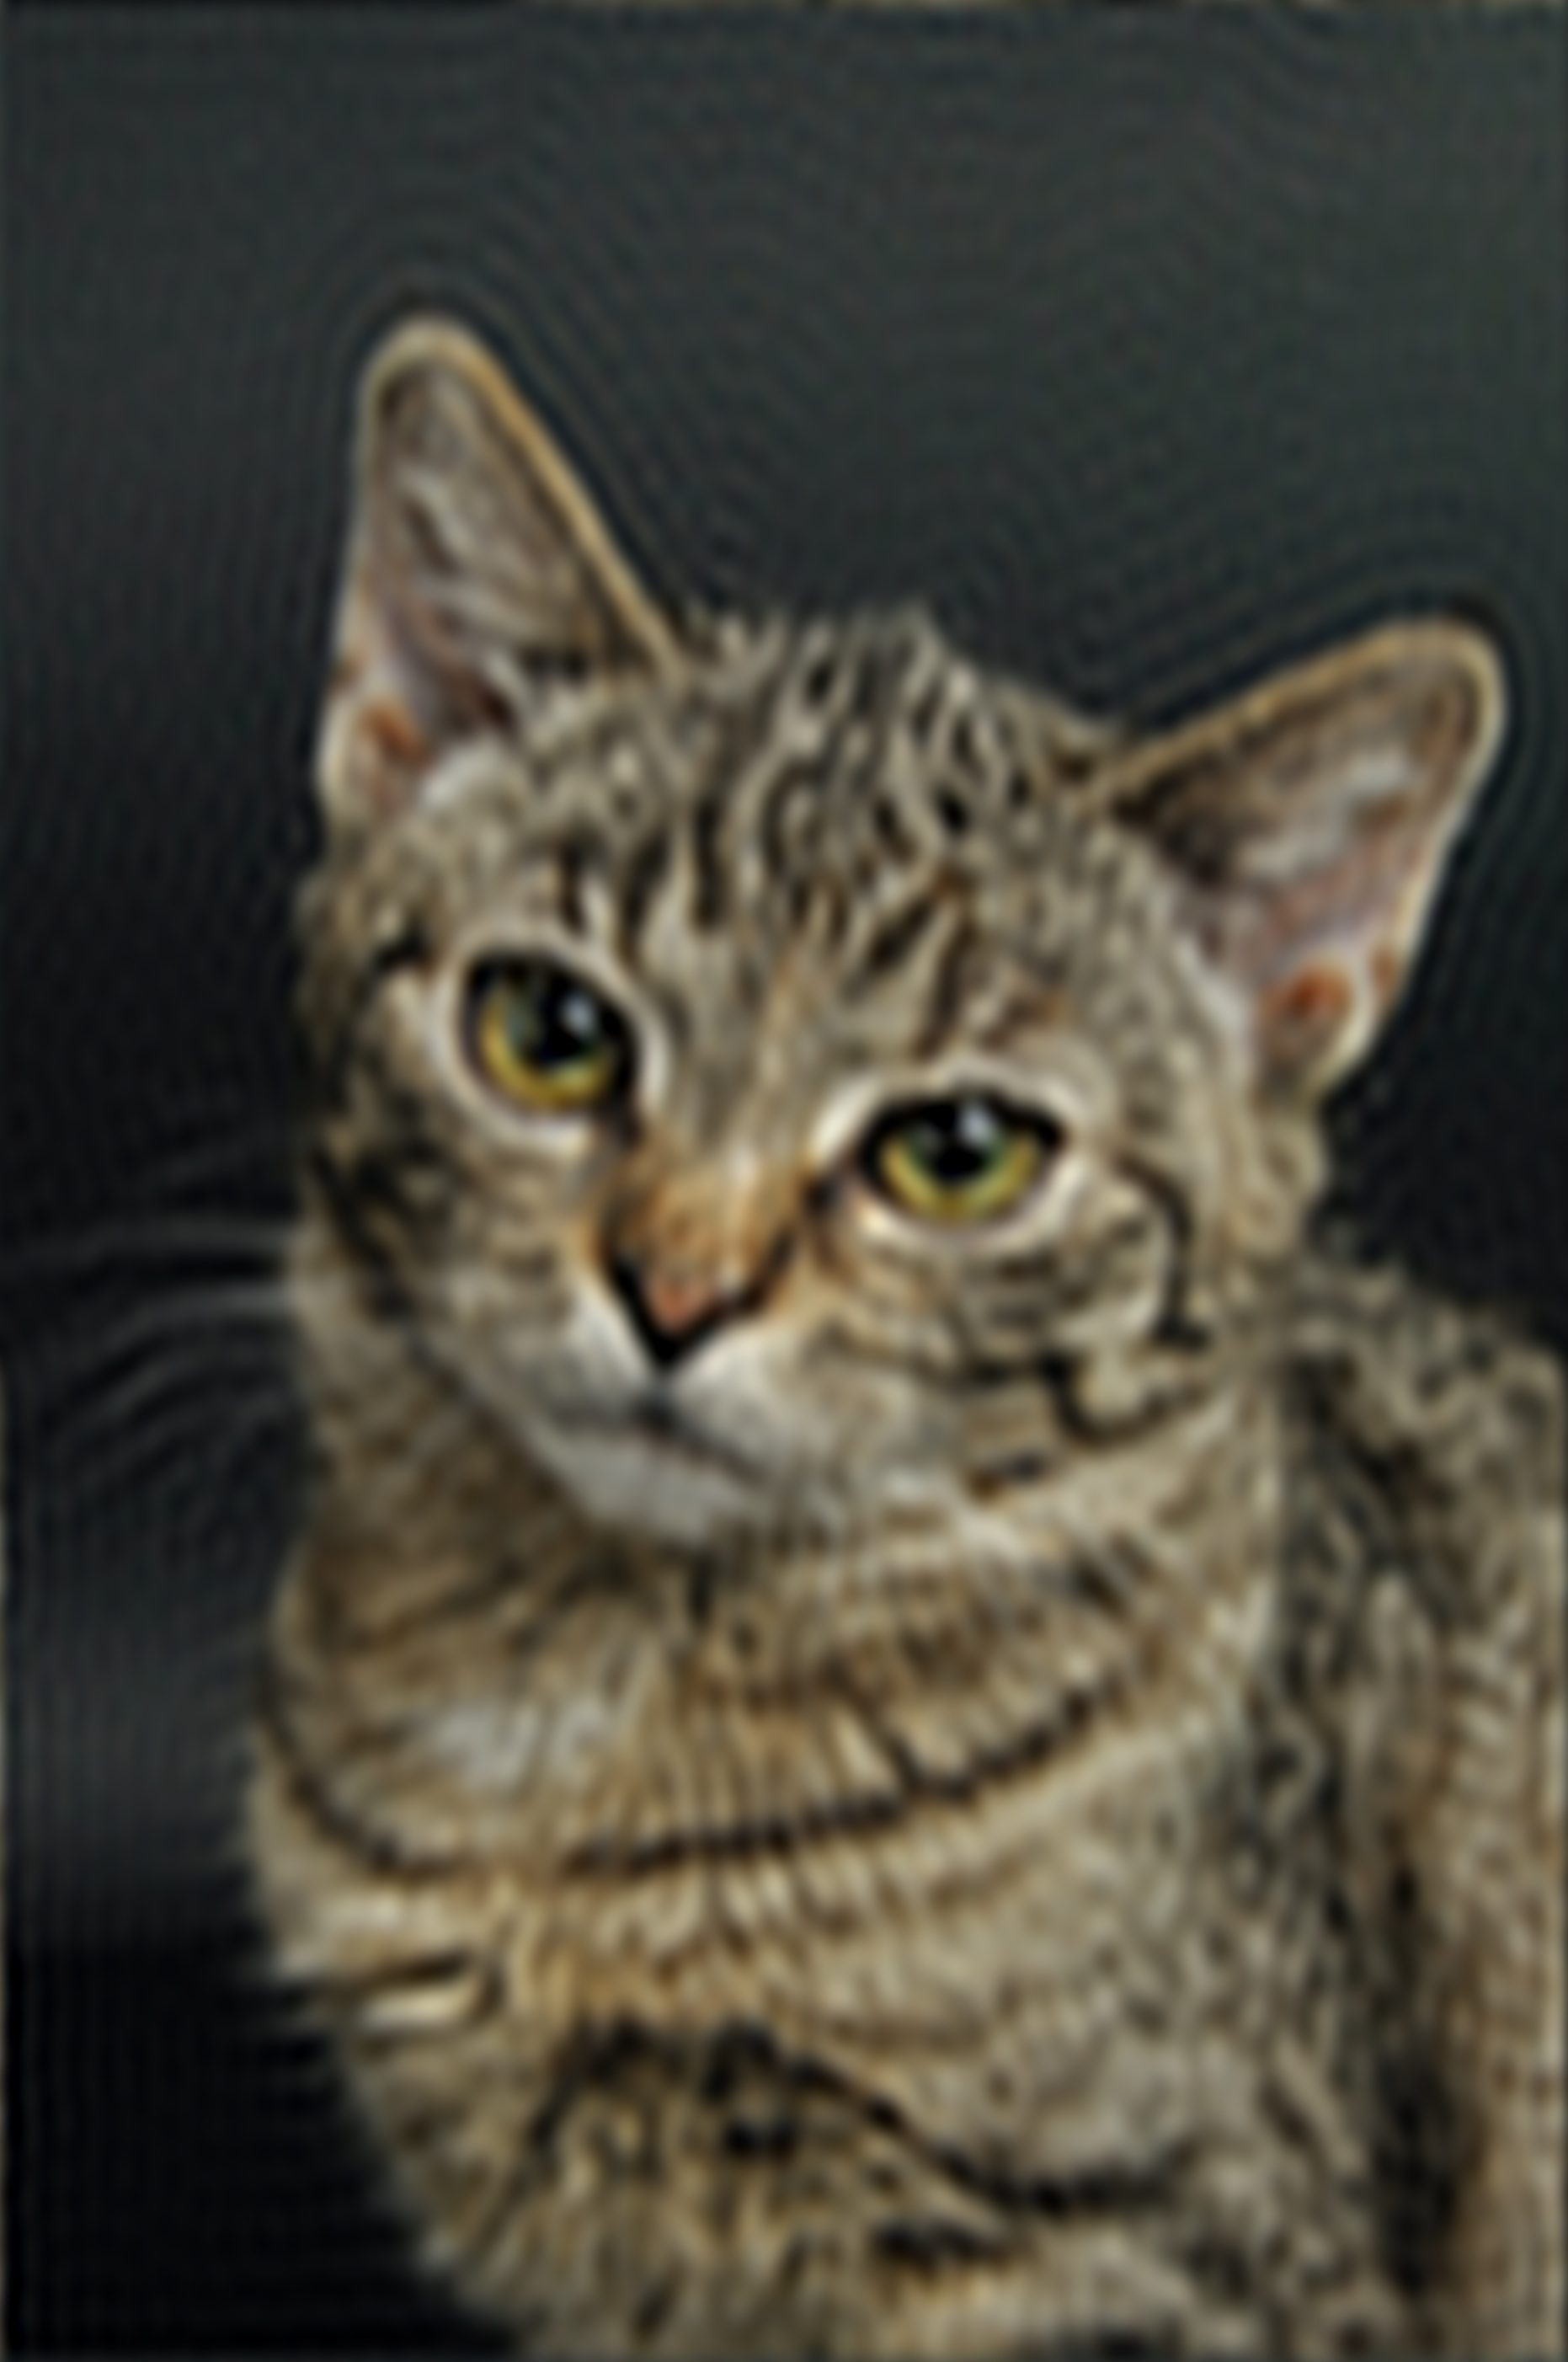
\includegraphics[keepaspectratio,height=0.7\textheight,width=1\textwidth]{output/ps2-5-a-2.jpg}}
                \captionof{figure}{ps2-5-a-2 resulting image}
            \end{minipage}
        
        	\begin{minipage}{0.45\textwidth}
        		\frame{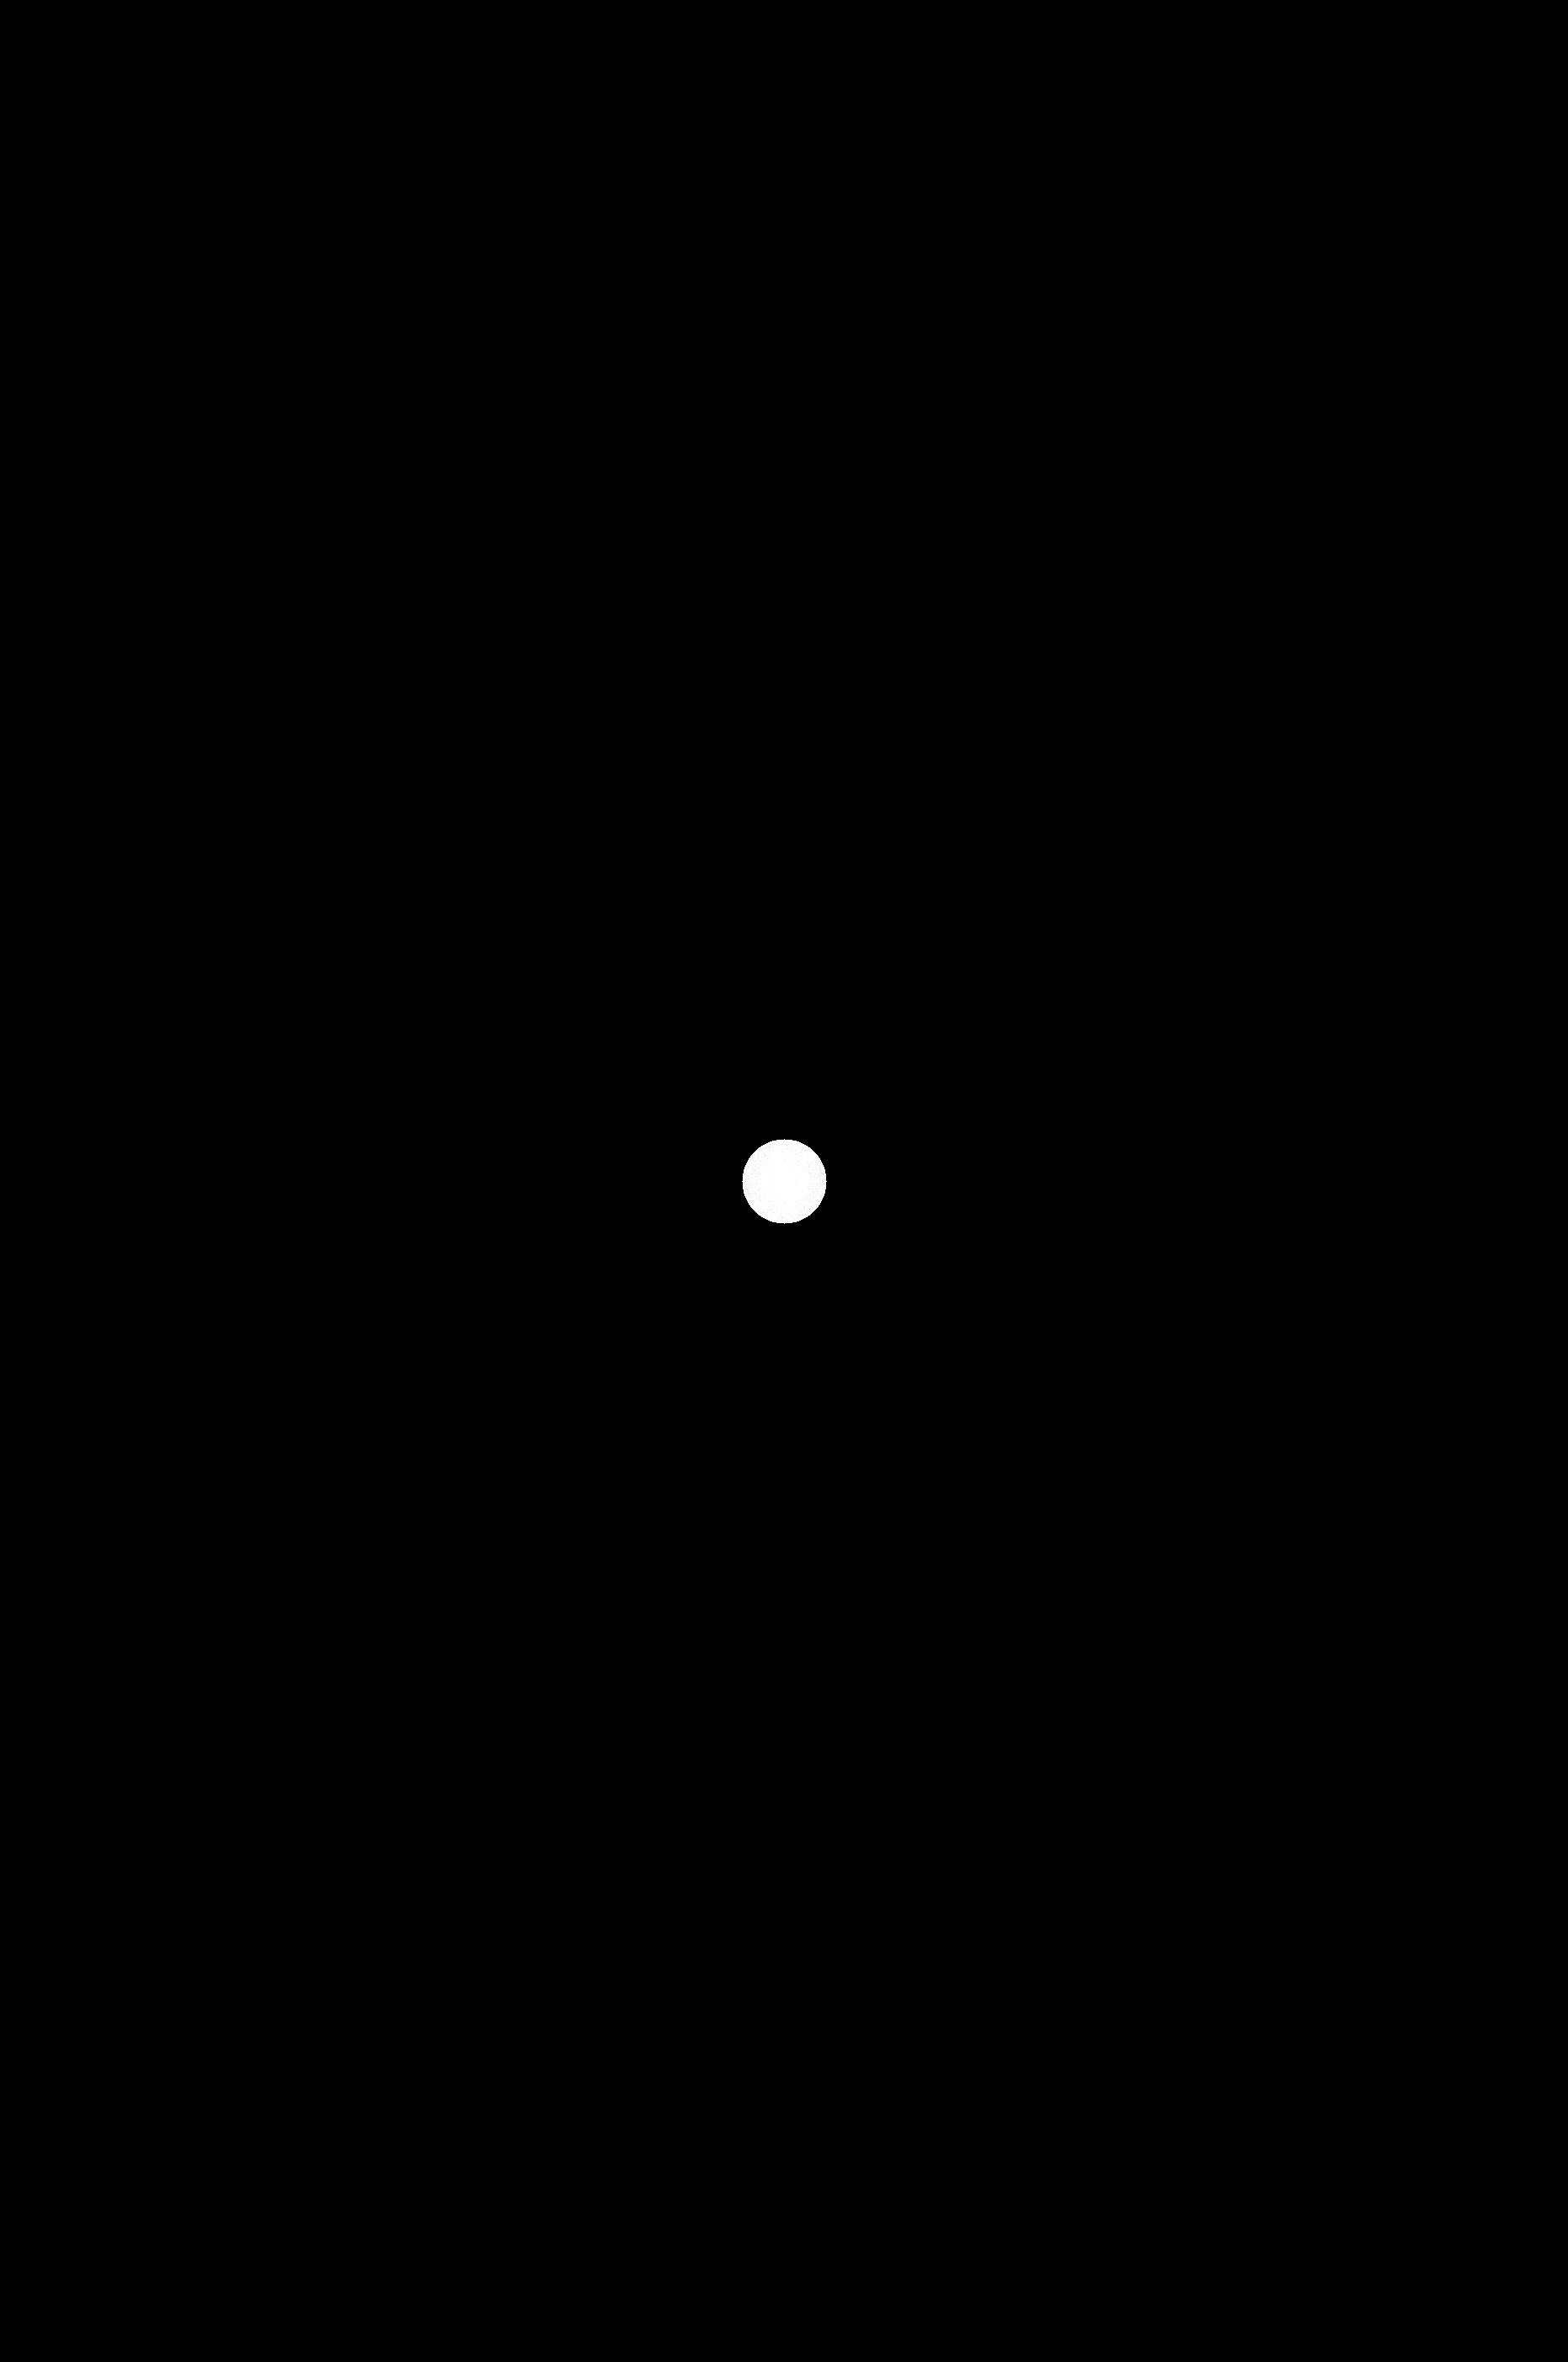
\includegraphics[keepaspectratio,height=0.7\textheight,width=1\textwidth]{output/ps2-5-a-2-freq.jpg}}
        		\captionof{figure}{ps2-5-a-2 frequency domain}
        	\end{minipage}
        
        \end{tabular}
        \end{table}
    \end{frame}
    
    \begin{frame}
    	\frametitle{5a3) Filtering - Radius 10}
    	\begin{table}[!htb]
        \centering
        \begin{tabular}{ c m{5cm} }
        
            \begin{minipage}{0.45\textwidth}
            \frame{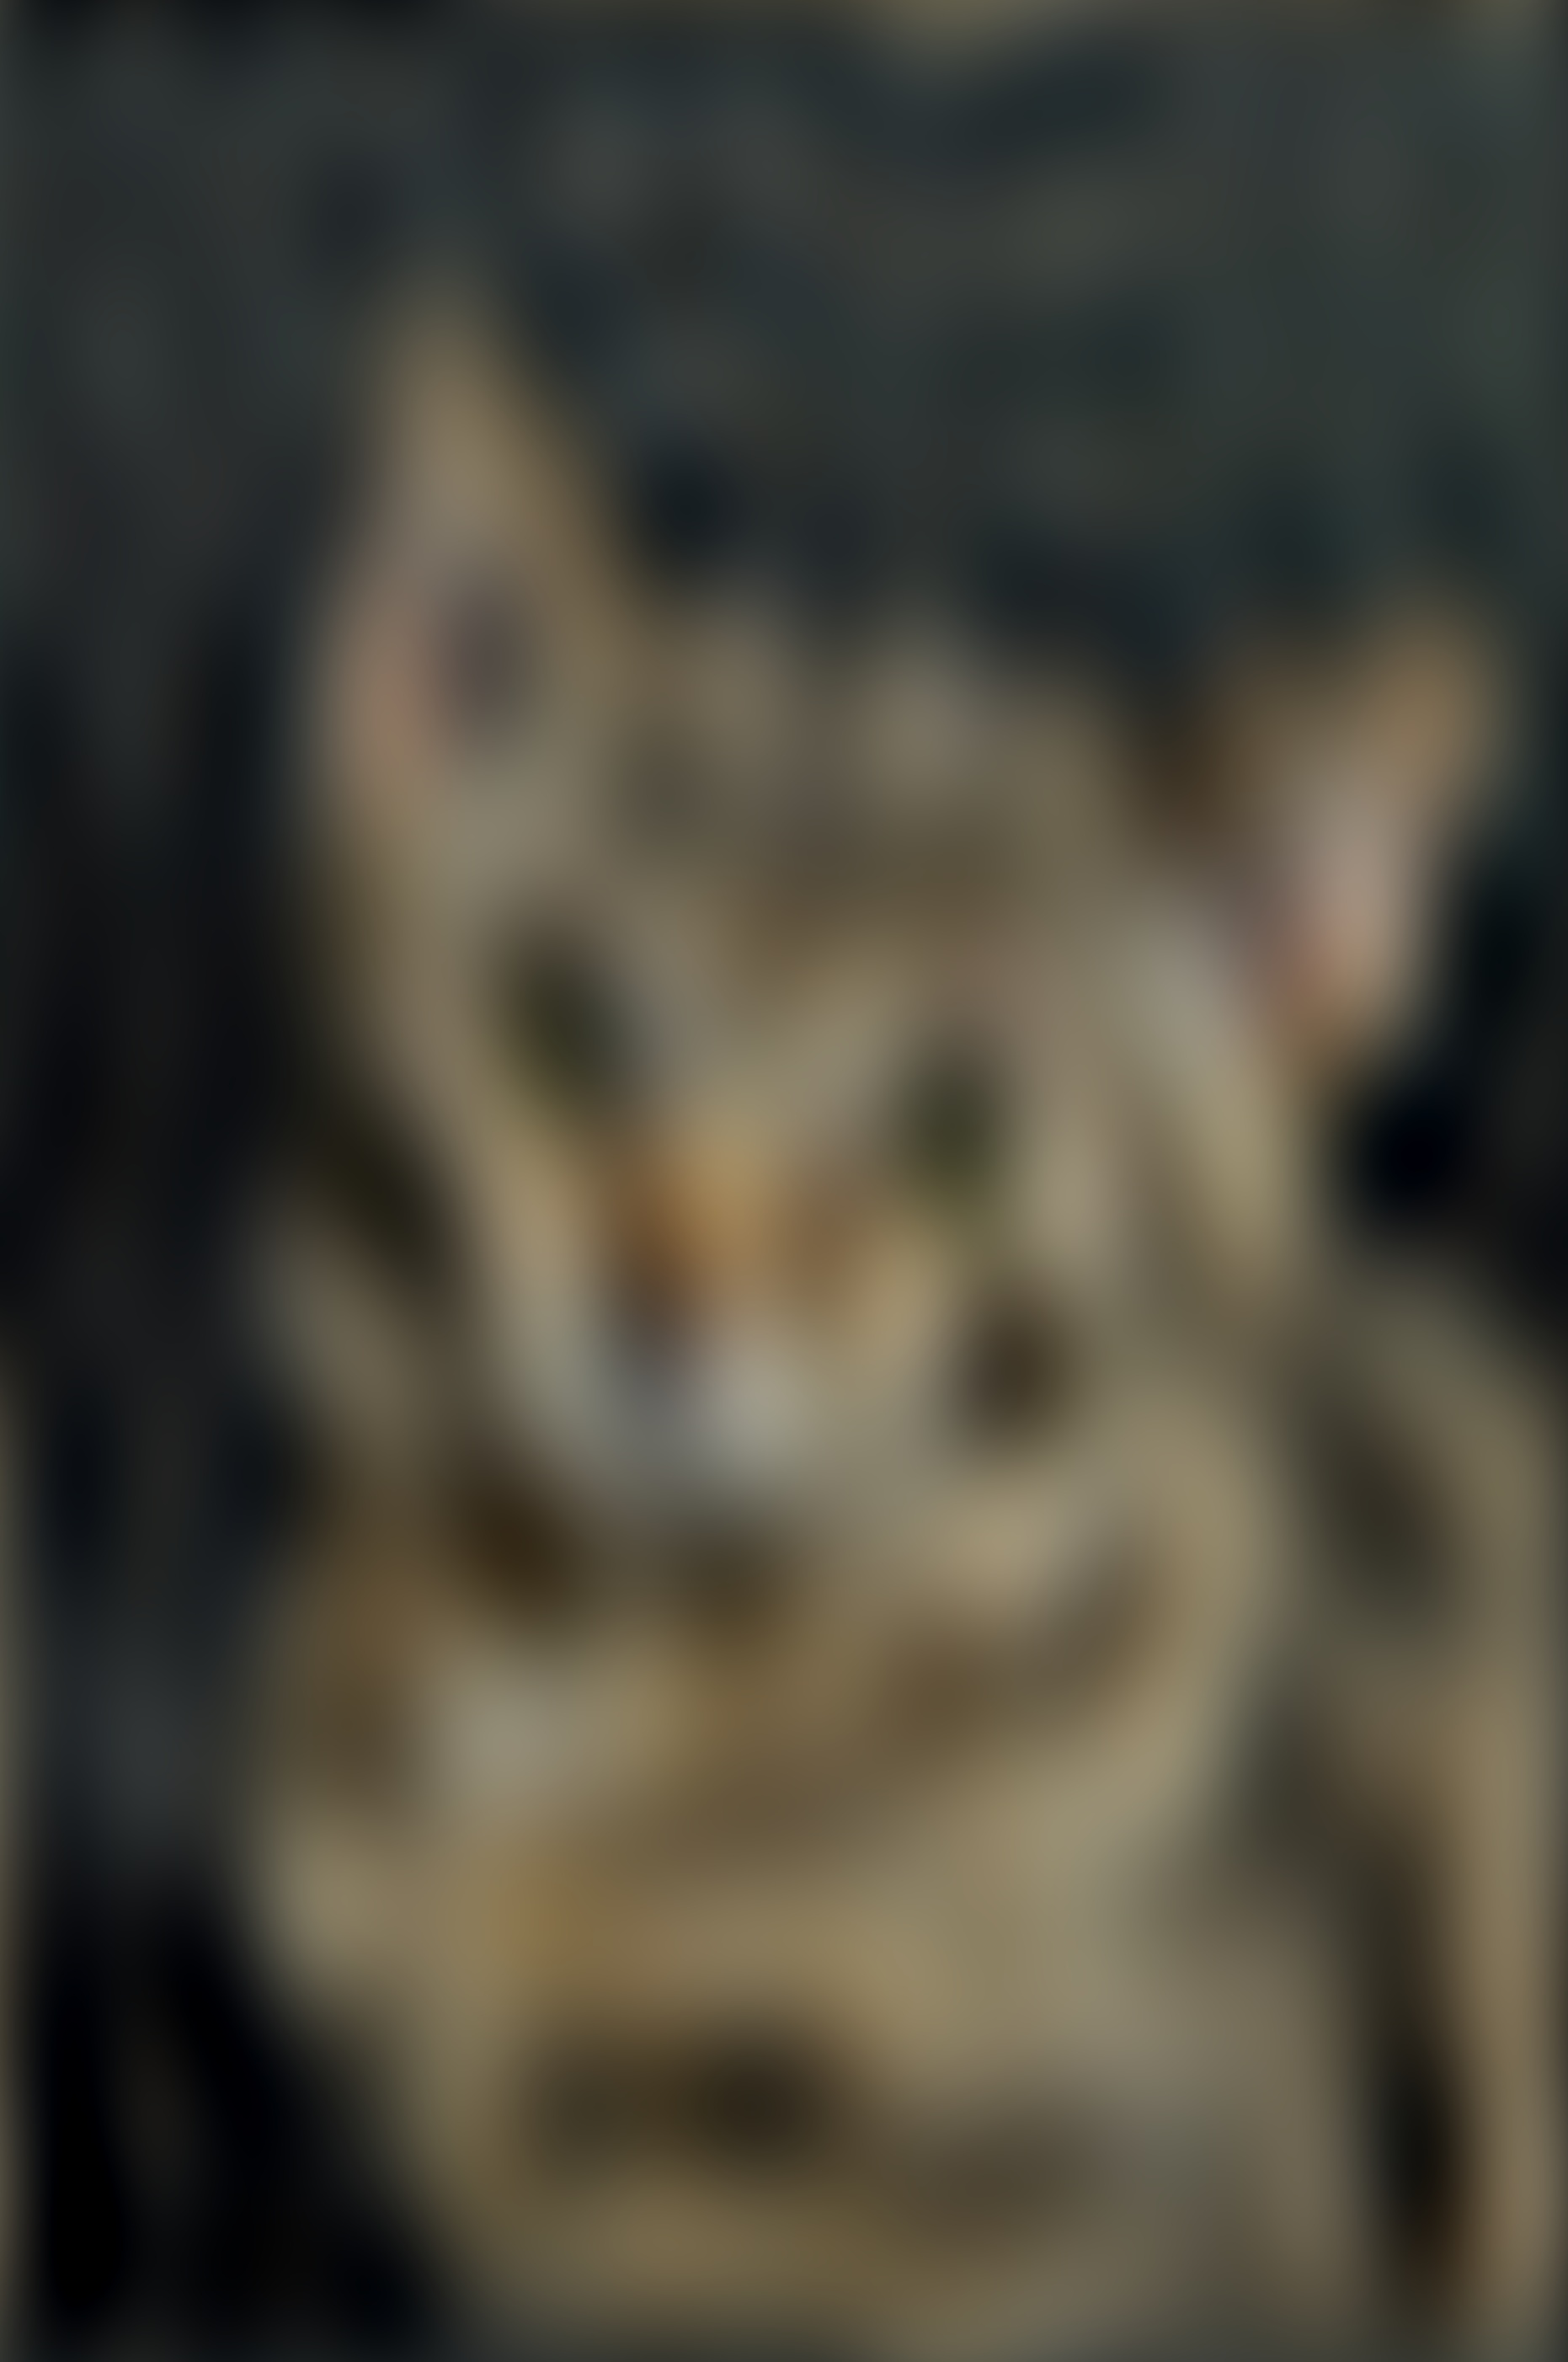
\includegraphics[keepaspectratio,height=0.7\textheight,width=1\textwidth]{output/ps2-5-a-3.jpg}}
                \captionof{figure}{ps2-5-a-3 resulting image}
            \end{minipage}
        
         	\begin{minipage}{0.45\textwidth}
        		\frame{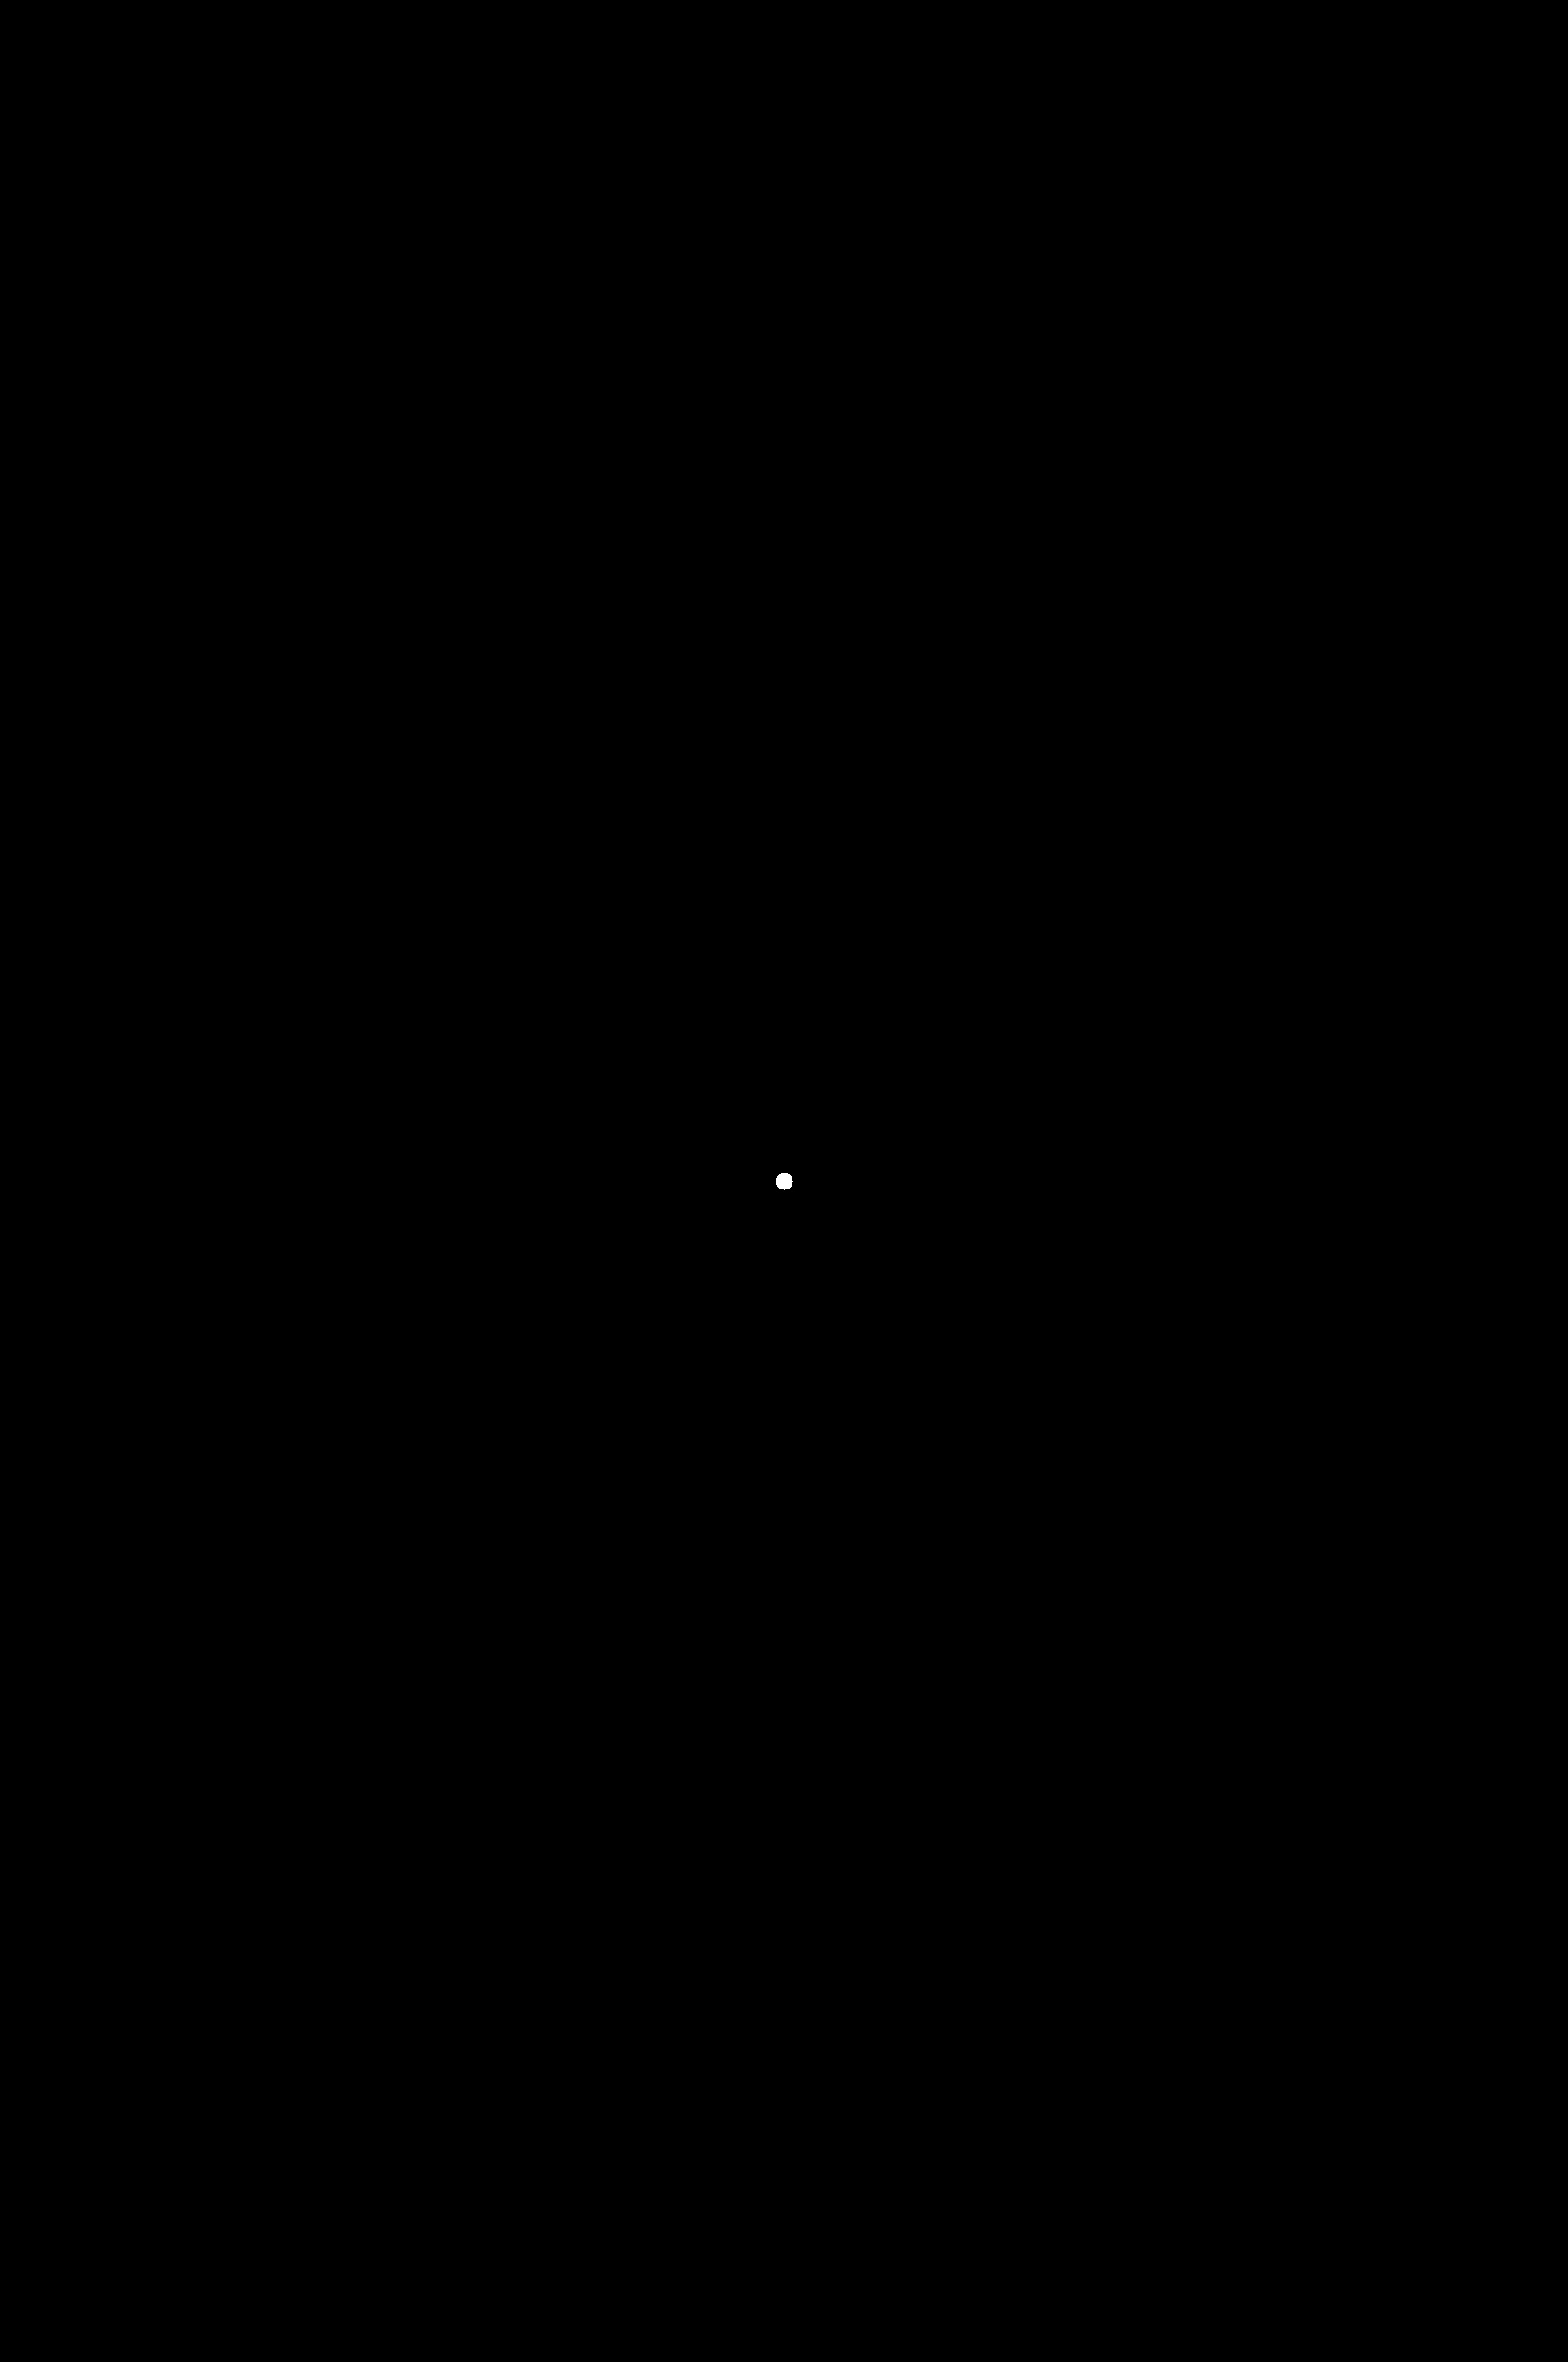
\includegraphics[keepaspectratio,height=0.7\textheight,width=1\textwidth]{output/ps2-5-a-3-freq.jpg}}
        		\captionof{figure}{ps2-5-a-3 frequency domain}
        	\end{minipage}
        
        \end{tabular}
        \end{table}
    \end{frame}
    
    \begin{frame}[t]
		\frametitle{5b) Discussion}
		
		\begin{normalsize}
			\begin{itemize}
				\setlength\itemsep{1em}\fontsize{6pt}{6pt}
				
				\item[] \textbf{
					What are the differences between compression and filtering? How does this change the resulting image?
				 }

				\item[] {\selectfont\textcolor{blue}{Answer here.}}

			\end{itemize}
		\end{normalsize}
		
	\end{frame}
	\begin{frame}[t]
		\frametitle{5c) Discussion}
		
		\begin{normalsize}
			\begin{itemize}
				\setlength\itemsep{1em}\fontsize{6pt}{6pt}
				
				\item[] \textbf{
					Given an image corrupted with salt and pepper pepper noise, what filtering method can effectively reduce/remove this noise? Also explain your choice of filtering method. 
				 }

				\item[] {\selectfont\textcolor{blue}{Answer here.}}

			\end{itemize}
		\end{normalsize}
		
	\end{frame}
\end{document}